% Template construction -- groupwise SyGN template with ANTsPy (build_template).
% Subsection of "Registration", pulled in by sections/04-registration.tex.
% Sources: SyN = avants2008syn, SyGN = avants2010sygn, implementation = ANTsPy (tustison2021antsx).
% Lines marked "TODO" need a value or a check from your own run / log file.

% ==============================================================================
\subsection[Template construction]{Template construction}
\label{sec:template}             % new label for this section

To obtain a common spatial reference for the pulmonary airway trees, a
population-specific three-dimensional template was constructed from airway
segmentation volumes using the Advanced Normalization Tools (ANTs) framework and
its ANTsPy interface \cite{tustison2021antsx}. Template construction is a
\emph{groupwise registration problem}: a common template and a set of
transformations mapping the individual airway trees to it are estimated
together. Unlike pairwise registration to an arbitrarily selected subject,
groupwise registration does not designate one individual airway tree as the
anatomical reference; the reference itself is progressively optimised to
represent the population. The ANTs framework implements this as \emph{symmetric
groupwise normalization} (SyGN) \cite{avants2010sygn}. The registration of
individual airway trees to the finished template is described separately in
\secref{sec:affine}.

\paragraph{Sources of the method description.}  % reader knows which claim comes from where
The description combines three sources. (i)~The pairwise deformable registration
algorithm, Symmetric Normalization (SyN), was introduced by
\citet{avants2008syn} (\secref{sec:syn}). (ii)~The groupwise
template-construction strategy, SyGN, was introduced by \citet{avants2010sygn}
(\secref{sec:sygn}). (iii)~The template initialisation, the appearance
update, the parameter defaults and the order of operations are properties of the
ANTsPy implementation (\texttt{ants.registration} and
\texttt{ants.build\_template}) \cite{tustison2021antsx}; where the implementation
differs from the published algorithms, this is stated explicitly. Both methods
were developed and validated on T1-weighted brain MRI (cortical labelling in
elderly and neurodegenerative brains, and hippocampus segmentation in epilepsy,
respectively); neither was evaluated on airway segmentations.

% ==============================================================================
\subsubsection{Input data and image geometry}
\label{sec:tpl_data}             % data selection, physical space, notation

\paragraph{Selection of the input volumes.}  % what went into build_template
Eight airway segmentation volumes were used: four drawn at random from ATM'22 and
four from AIIB23 (\secref{sec:datasets}). The draw used Python's
pseudo-random generator without a fixed seed, so the selected subset is not
reproducible from the code alone; the file names were recorded in the run log
and are listed in Table~\ref{tab:template_inputs}.
\begin{table}[htbp]              % the 8 volumes given to ants.build_template
  \centering                     % centre the table
  \caption{Airway segmentations used to build the template, in input order.}
  \label{tab:template_inputs}    % referenced in "Selection of the input volumes"
  \begin{tabular}{clll}          % order, dataset, file name
    \toprule
    Order & Dataset & File name \\
    \midrule
    1 & ATM'22 & \TODO{file name} \\
    2 & ATM'22 & \TODO{file name} \\
    3 & ATM'22 & \TODO{file name} \\
    4 & ATM'22 & \TODO{file name} \\
    5 & AIIB23 & \TODO{file name} \\
    6 & AIIB23 & \TODO{file name} \\
    7 & AIIB23 & \TODO{file name} \\
    8 & AIIB23 & \TODO{file name} \\
    \bottomrule
  \end{tabular}
\end{table}
% TODO: fill in the 8 file names from the run log,
% TODO: or set `seed` in run_template_registration.py and report it here.
The volumes were passed to \texttt{ants.build\_template} in the order ATM'22
first, then AIIB23. This order matters for one implementation detail: the first
volume defines the voxel grid of the template (see \emph{Initialisation} in
\secref{sec:sygn}).

\paragraph{Representation in physical space.}  % voxel index vs physical coordinate
Each airway tree is a three-dimensional NIfTI image: a discrete voxel array
together with spatial metadata that positions the array in physical space. A
voxel is identified by a discrete index $\mathbf{i}=(i_x,i_y,i_z)^T$, whereas its
anatomical location is a continuous physical coordinate
$\mathbf{x}=(x,y,z)^T$, related by
\begin{equation}
  \mathbf{x} = \mathbf{o} + \mathbf{D}
  \begin{bmatrix}
    s_x & 0   & 0   \\
    0   & s_y & 0   \\
    0   & 0   & s_z
  \end{bmatrix}
  \mathbf{i},
  \label{eq:index_to_physical}   % voxel index -> physical coordinate
\end{equation}
where $\mathbf{o}$ is the image origin, $s_x,s_y,s_z$ are the voxel spacings and
$\mathbf{D}$ is the direction matrix of the voxel axes; in NIfTI terminology these
are encoded by the spatial affine in the image header. ANTs is built on ITK, in
which registration is performed in \emph{physical coordinates}, and ANTsPy
converts the NIfTI geometry into the ITK representation of origin, spacing and
direction. Differences in origin, orientation or voxel spacing between two
airway segmentations are therefore taken into account when their structures are
put into correspondence. The NIfTI affine defines the \emph{initial coordinate
system of each image}; it is not itself a registration.

\paragraph{Warping convention.}  % direction of the maps used in all equations below
An image $I$ is treated as a function of physical position, and a transformation
is applied by composition. If $T$ is the fixed image (the template) and $I$ the
moving image, the warped image is defined on the domain of $T$:
\begin{equation}
  (I\circ\Phi)(\mathbf{x}) = I\big(\Phi(\mathbf{x})\big),
  \qquad \mathbf{x}\in\Omega_T .
  \label{eq:pullback}            % warping = resampling the moving image at mapped points
\end{equation}
Hence $\Phi$ maps each point of the \emph{template} domain to its corresponding
point in the \emph{subject} domain, where the subject image is resampled. This is
the convention used by ITK and ANTs; the inverse map $\Phi^{-1}$ takes subject
points to template points.

% ==============================================================================
\subsubsection{Pairwise registration with SyN}
\label{sec:syn}                  % one registration call inside the template loop

% think about saying 

% At the first template-building call, no template is supplied. 
% ANTsPy therefore constructs an initial template by equally weighting and averaging the 
% input images after resampling them to a common image geometry. This preliminary average is
% then used as the fixed image for the first set of pairwise SyN registrations. 
% The resulting warped images and estimated transformations are subsequently used to update the template.
% In subsequent calls, the template from the preceding iteration is supplied as initial_template and serves 
% as the starting point for the next iteration.

Within every template-building iteration $k$, each airway segmentation $I_i$ is
registered to the current template $T^{(k)}$, which serves as the fixed image.
The registration seeks $\Phi_i^{(k)}$ such that
\begin{equation}
  I_i \circ \Phi_i^{(k)} \approx T^{(k)},
  \label{eq:registration_goal}   % warped subject should resemble the template
\end{equation}
i.e.\ after warping, corresponding airway structures occupy similar physical
locations in template space. Inside \texttt{ants.build\_template} this is the call

\begin{lstlisting}
ants.registration(
    fixed=xavg,        # current template T^(k)
    moving=image_i,    # airway segmentation I_i
    type_of_transform='SyN'
)
\end{lstlisting}

\paragraph{The ANTsPy \texttt{SyN} preset.}  % what the preset contains
Despite its name, the ANTsPy preset \texttt{SyN} contains three stages. The two
images are first aligned by their centres of mass (a translation used as initial
transform), an affine transformation $A_i^{(k)}$ is then estimated, and finally
the deformable symmetric normalisation $\phi_i^{(k)}$ is estimated between the
template and the affinely transformed subject $I_i\circ A_i^{(k)}$. In
\citet{avants2008syn}, by contrast, ``SyN'' denotes only the deformable part, and
rigid and scaling differences are assumed to have been removed beforehand. With
the convention of Eq.~\eqref{eq:pullback}, the total transformation is
\begin{equation}
  \Phi_i^{(k)} = A_i^{(k)} \circ \phi_i^{(k)},
  \qquad
  I_i\circ\Phi_i^{(k)} = \big(I_i\circ A_i^{(k)}\big)\circ\phi_i^{(k)},
  \label{eq:affine_plus_syn}     % template point -> deformable -> affine -> subject point
\end{equation}
so a template point is moved first by the deformable map and then by the affine
map into subject space. The affine part accounts for global translation,
rotation, scaling and shear; the deformable part accounts for spatially varying
differences that no single affine map can represent. (The centre-of-mass
translation is folded into the affine stage.)

\paragraph{Registration parameters.}  % values needed to reproduce the registration
Apart from \texttt{type\_of\_transform}, no argument was specified, so all
other settings were ANTsPy defaults: Mattes mutual information as the similarity metric of both the
affine and the deformable stage; an affine stage with
$(2100,1200,1200,10)$ iterations on four resolution levels; a deformable stage
with $(40,20,0)$ iterations from coarse to fine; an optimiser step
\texttt{grad\_step} $=0.2$; and Gaussian smoothing of the update field
(\texttt{flow\_sigma} $=3$) and of the total field (\texttt{total\_sigma} $=0$).
Because the last entry of the deformable iterations is zero, no deformable
optimisation is performed at full image resolution, which limits how precisely
thin peripheral airway branches can be aligned. The SyN step \texttt{grad\_step}
is unrelated to the template shape-update step \texttt{gradient\_step} of
\secref{sec:sygn}, although both equal $0.2$.
% TODO: the defaults above were read from the ANTsPy source (master branch);
% TODO: check them against the ANTsPy version printed at the top of your run log.

\paragraph{Similarity metric.}  % where the pipeline differs from both papers
Mutual information (MI) measures the statistical dependence between the
intensity distributions of the fixed and warped moving image, estimated from
their joint histogram. It is \emph{not} the metric used in either reference
publication. \citet{avants2008syn} developed SyN with \emph{local
cross-correlation} (CC), arguing that MI is a global measure well suited to
rigid registration but potentially limiting for deformable registration, and
that a localised MI estimate becomes unreliable because joint probabilities need
many samples; local CC depends only on local means and variances, which can be
estimated from few samples. SyGN \cite{avants2010sygn} likewise uses local CC
both for the registrations and for the template appearance. With the
mean-subtracted images $\bar I = I-\mu_I$ and $\bar J = J-\mu_J$, the means being
computed in a small cubic neighbourhood of $\mathbf{x}$, local CC is
\begin{equation}
  CC(\bar I,\bar J,\mathbf{x})
  = \frac{\langle \bar I,\bar J\rangle^2}
         {\langle \bar I,\bar I\rangle\,\langle \bar J,\bar J\rangle},
  \label{eq:local_cc}            % inner products over the same neighbourhood
\end{equation}
with inner products over the same neighbourhood ($5^3$ voxels in
\citet{avants2008syn}, radius 4 in \citet{avants2010sygn}). Because the airway
volumes are segmentations, any metric compares the spatial patterns of the
label values rather than anatomical intensities.
% TODO: optionally justify MI for binary masks, or compare with syn_metric='CC' / 'meansquares'.

\paragraph{Registration as optimisation.}  % how SyN differs from elastic registration
Deformable registration is often written as
\begin{equation}
  \hat{\Phi} = \arg\min_{\Phi}\;
  D\!\left(T,\, I\circ\Phi\right) + \lambda\, R(\Phi),
  \label{eq:registration_objective}  % generic data term + weighted regulariser
\end{equation}
with a dissimilarity term $D$, a regulariser $R$ and a weight $\lambda$. This is
the classical elastic formulation. SyN departs from it: \citet{avants2008syn}
restrict the search to diffeomorphisms and optimise the similarity term
essentially without a competing penalty. Regularity comes from the diffeomorphic
path structure and from smoothing of the velocity field; the regularisation term
contributes little to the total energy but ensures that a path of minimal length
is found.

\paragraph{Diffeomorphisms generated by velocity fields.}  % the basic building block
A diffeomorphism is a differentiable map with a differentiable inverse. In SyN,
as in other large-deformation methods, it is generated by integrating a
time-dependent velocity field $\mathbf{v}(\mathbf{x},t)$:
\begin{equation}
  \frac{\partial \phi(\mathbf{x},t)}{\partial t}
  = \mathbf{v}\big(\phi(\mathbf{x},t),\,t\big),
  \qquad
  \phi(\mathbf{x},0) = \mathbf{x}.
  \label{eq:syn_flow}            % flow ODE starting from the identity
\end{equation}
The regularity of $\mathbf{v}$ is measured by a norm $\|\mathbf{v}\|_L$ induced
by a linear differential operator such as $L=a\nabla^2+b\,\mathrm{Id}$, and the
path length
\begin{equation}
  D\big(\phi(\cdot,0),\phi(\cdot,1)\big)
  = \int_0^1 \|\mathbf{v}(\cdot,t)\|_L\,dt
  \label{eq:shape_distance}      % geodesic (shape) distance between two images
\end{equation}
defines a distance between shapes; its infimum over admissible velocity fields is
a true metric, whose shortest paths are geodesics. This distance is what SyGN
later minimises to find the average shape (\secref{sec:sygn}).

\paragraph{Symmetric two-part formulation.}  % the core idea of SyN
SyN splits the path between two images $I$ and $J$ into two halves. Two
diffeomorphisms, $\phi_1$ acting on $I$ and $\phi_2$ acting on $J$, are generated
by Eq.~\eqref{eq:syn_flow} with their own velocity fields, each integrated from
the identity only over $t\in[0,0.5]$. The two images are deformed towards each
other and compared at the midpoint (figure~\ref{fig:syn_path}):
\begin{equation}
  \begin{split}
    E_{S}(I,J) = \inf_{\phi_1}\inf_{\phi_2}\;
      & \int_{0}^{0.5}
        \Big( \|\mathbf{v}_1(\cdot,t)\|_L^2 + \|\mathbf{v}_2(\cdot,t)\|_L^2 \Big)\,dt \\
      & + \int_{\Omega}
        \Pi\big( I\circ\phi_1(\cdot,0.5),\; J\circ\phi_2(\cdot,0.5) \big)\,d\Omega ,
  \end{split}
  \label{eq:syn_energy}          % SyN energy: two half-path lengths + midpoint dissimilarity
\end{equation}

  % first mention, right after Eq. syn_energy

\begin{figure}[htbp]                                   % float near the SyN paragraph
  \centering                                           % centre the image
  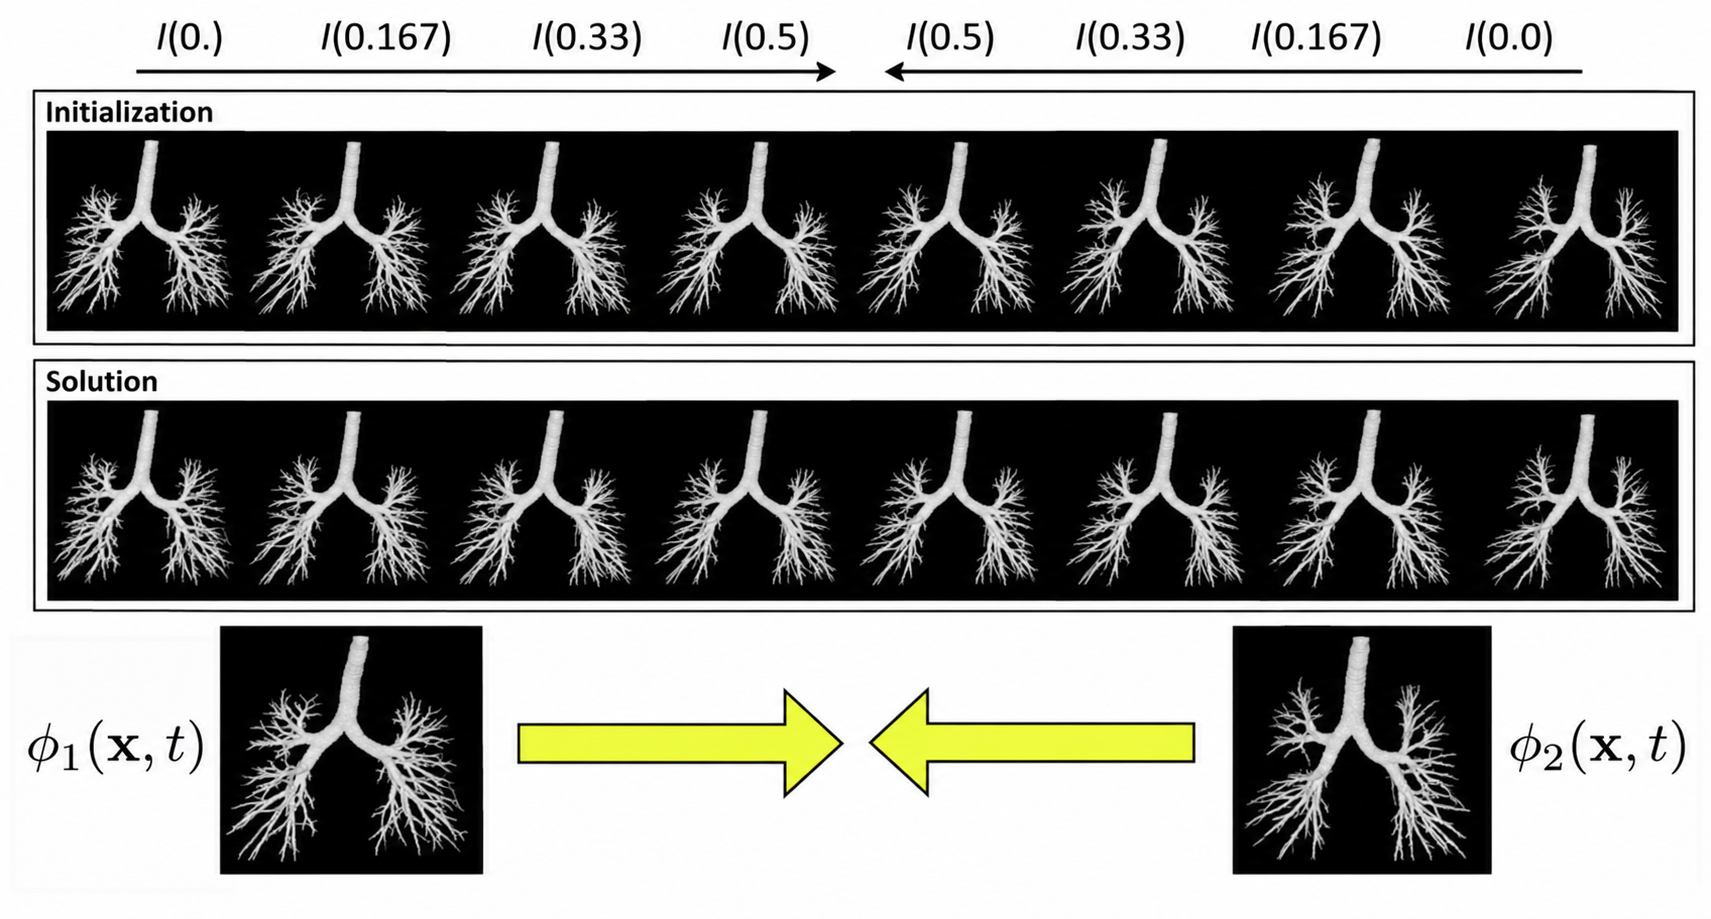
\includegraphics[width=\textwidth]{figures/syn_path_airways.png}  % the uploaded image
  \caption{Schematic of the symmetric SyN path between two airway trees $I$
  (left) and $J$ (right).
  Top: the two images at initialisation. Middle: after convergence, both
  images are deformed along $\phi_1$ and $\phi_2$ and meet at the mean shape
  at $t=0.5$. The full map from $I$ to $J$ is obtained by joining the two
  half-paths (Eq.~\ref{eq:syn_composition}). Illustrative only; not
  computed from the study data.}
  \label{fig:syn_path}                                 % referenced in the text above
\end{figure}

where $\Pi$ is a pointwise dissimilarity (the squared intensity difference in the
derivation of \citet{avants2008syn}, $-CC$ in their main method). The two
half-paths are kept at equal length, so both images travel the same distance and
meet at the \emph{mean shape} between them; SyN thus solves a two-image mean
problem, the pairwise counterpart of the template estimation in
\secref{sec:sygn}.

\paragraph{Full transformations by composition.}  % how the time-1 maps are obtained
The complete mapping between the two images is obtained by joining the
half-paths:
\begin{equation}
  \phi_1(\mathbf{x},1) = \phi_2^{-1}\big(\phi_1(\mathbf{x},0.5),\,0.5\big),
  \qquad
  \phi_1^{-1}(\mathbf{x},1) = \phi_1^{-1}\big(\phi_2(\mathbf{x},0.5),\,0.5\big).
  \label{eq:syn_composition}     % forward and inverse maps from the two halves
\end{equation}
Because $I$ and $J$ enter Eq.~\eqref{eq:syn_energy} in the same way, exchanging
them yields the same path in the opposite direction: the result does not depend
on which image is called ``fixed'' and which ``moving''.

\paragraph{Explicit, accurate inverses.}  % what distinguishes SyN from inverse-consistent methods
Diffeomorphisms are invertible in the continuous setting, but interpolation
errors in a discrete implementation accumulate and can break invertibility. SyN
therefore computes the inverses $\phi_i^{-1}$ explicitly with a fixed-point
algorithm and enforces $\phi_i^{-1}(\phi_i)=\mathrm{Id}$ and
$\phi_i(\phi_i^{-1})=\mathrm{Id}$ to sub-voxel accuracy. This distinguishes SyN
from inverse-consistent registration, in which forward and backward maps are
estimated separately and made consistent only approximately through penalty
terms. Both the subject-to-template and the template-to-subject mappings are
therefore available and consistent.

\paragraph{Optimisation in practice.}  % the algorithmic loop of one registration
Each SyN iteration deforms both images to the midpoint, computes the gradient of
the similarity term with respect to each half-map, smooths it into velocity
updates, updates $\phi_1$ and $\phi_2$ through a discretisation of
Eq.~\eqref{eq:syn_flow} with a sub-voxel step, recomputes the inverses and forms
the maps of Eq.~\eqref{eq:syn_composition}. The operator $L$ is approximated by a
Gaussian kernel applied to the \emph{incremental} update rather than to the total
displacement (\texttt{flow\_sigma} and \texttt{total\_sigma} in ANTsPy);
smoothing the increment is what permits large diffeomorphic deformations,
whereas smoothing the total displacement, as in elastic and Demons-type methods,
restricts the solution to small deformations. The optimisation runs from coarse
to fine resolution levels.
% TODO: current ANTs releases implement a greedy variant of SyN; cite the ANTs
% TODO: implementation paper if you want to state this explicitly.

% ==============================================================================
\subsubsection{Groupwise template construction with SyGN}
\label{sec:sygn}                 % the build_template loop

\paragraph{Formulation.}  % what SyGN optimises (avants2010sygn, Eq. 4)
SyGN seeks the template and the set of transformations that give the
``smallest'' parameterisation of the dataset, measured by the SyN energy of
Eq.~\eqref{eq:syn_energy}. The template is described by an appearance $\bar I$
(its intensities) and a shape, represented by a diffeomorphism $\psi$ that
defines the template's coordinate system. Given the images $\{J^i\}_{i=1}^N$,
\citet{avants2010sygn} minimise
\begin{equation}
  E_{\bar I} = \sum_{i=1}^{N} E_S\big(\bar I, J^i, \phi^i\big)
  \qquad\text{with}\qquad \phi^i(\mathbf{x},0) = \psi(\mathbf{x})\;\;\forall i,
  \label{eq:sygn_energy}         % sum of pairwise SyN energies, common starting point psi
\end{equation}
jointly over the mappings $\phi^i$, the appearance $\bar I$ and the shape $\psi$.
No initial template has to be chosen by the user, and the stated goals are that
the final template's appearance does not depend on any specific anatomy and its
shape does not depend on any individual's coordinate system.

\paragraph{Coordinate-descent algorithm.}  % the loop in the paper
Eq.~\eqref{eq:sygn_energy} is minimised by coordinate descent, one group of
variables at a time with the others fixed. After initialisation, each iteration
(1)~registers every image to the fixed template with SyN; (2)~updates the template
appearance $\bar I$; (3)~updates the template shape $\psi$ towards the average of
the mappings; and (4)~resamples the template through the new $\psi$, resets the
mappings to start from it, and repeats. The template is only updated after all
registrations of an iteration are complete, so appearance and shape are never
estimated from partially optimised mappings. \texttt{ants.build\_template}
implements the same loop, but with a different initialisation and a different
appearance update, as described next (figure~\ref{fig:sygn_paths}).

\begin{figure}[htbp]                                   % float near the SyGN loop
  \centering                                           % centre the image
  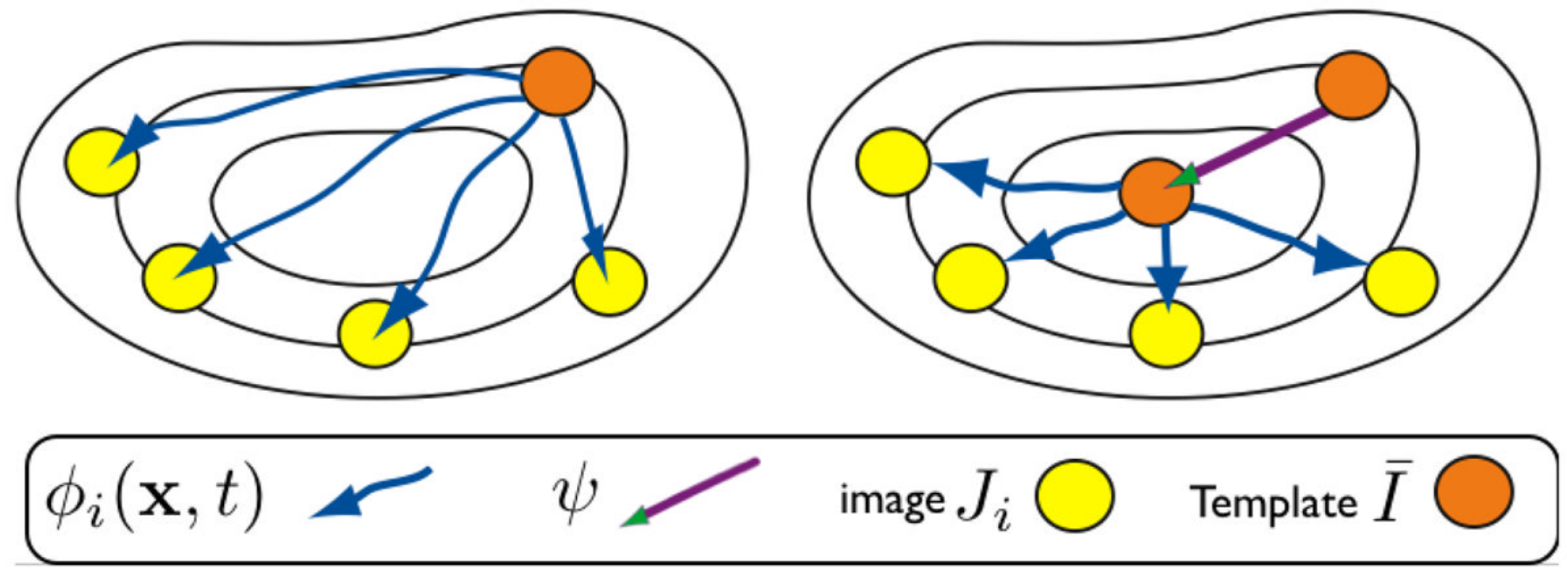
\includegraphics[width=0.8\textwidth]{figures/sygn_paths.png}  % Fig. 2 of avants2010sygn
  \caption{Two steps of one SyGN iteration. Left: the diffeomorphic paths
  $\phi_i$ from the current template $\bar I$ (orange) to the images $J_i$
  (yellow) are estimated (Step~1). Right: the template shape is moved by $\psi$
  towards the population centre, which shortens the total path length
  (Step~3). Reproduced from \citet{avants2010sygn}, Fig.~2.}
  \label{fig:sygn_paths}                               % referenced here and in Step 3
\end{figure}

\paragraph{Initialisation.}  % paper vs ANTsPy, and where the template grid comes from
In \citet{avants2010sygn}, the first template is the voxelwise (Euclidean)
average of the images \emph{after affine alignment}, and all $\phi^i$ and $\psi$
start as the identity. In the present implementation no initial template was
supplied, and ANTsPy forms the initial template \emph{without any alignment}: each
image is multiplied by its weight $w_i = 1/N$, resampled onto the voxel grid of
the first input image $I_1$, and summed,
\begin{equation}
  T^{(0)}(\mathbf{x}) = \sum_{i=1}^{N} w_i\, I_i(\mathbf{x}),
  \qquad \mathbf{x}\in\Omega_{I_1}.
  \label{eq:initial_template}    % unaligned mean, on the grid of the first image
\end{equation}
Two consequences follow. First, $T^{(0)}$ averages the airway trees as they lie
in their own scanner coordinates, so it is blurred and its quality depends on how
well these coordinate systems already agree. Because the inputs are binary
segmentations, it also contains intermediate values equal to the fraction of
volumes that contain airway at each location. Second, every later template is
resampled on this grid, so the origin, spacing, orientation and field of view of
the final template are inherited from $I_1$, here the first randomly selected
ATM'22 volume. The template's \emph{shape} is still optimised over the whole
population, but its \emph{grid} is not independent of the input order.

\paragraph{Step 1 -- registration.}  % links to the SyN subsection
With $T^{(k)}$ fixed, each $I_i$ is registered to it with the ANTsPy \texttt{SyN}
preset (\secref{sec:syn}), giving the affine maps $A_i^{(k)}$, the
deformable maps $\phi_i^{(k)}$ and the warped images
$I_i\circ\Phi_i^{(k)}$, all on the template grid.

\paragraph{Step 2 -- appearance update.}  % largest difference between paper and ANTsPy
\citet{avants2010sygn} do not take the template appearance to be a plain average.
They optimise it by gradient ascent on the cross-correlation of
Eq.~\eqref{eq:local_cc} between the template and the warped images (intensities
normalised to $[0,1]$, gradients smoothed with a Gaussian of $\sigma=1$ voxel,
step size $0.1$), and show that this preserves more contrast and detail than the
Euclidean mean. ANTsPy does \emph{not} implement this step. Its appearance is the
weighted Euclidean mean of the warped images,
\begin{equation}
  T_{\mathrm{avg}}^{(k+1)}(\mathbf{x})
  = \sum_{i=1}^{N} w_i \left[ I_i\circ\Phi_i^{(k)} \right]\!(\mathbf{x}),
  \label{eq:average_registered}  % mean of the aligned (warped) airway images
\end{equation}
and, at the end of each iteration (after the shape update below), this image is
blended with a sharpened copy of itself,
\begin{equation}
  T^{(k+1)} = \beta\, T^{(k+1)}_{\mathrm{shape}}
  + (1-\beta)\, \operatorname{Sharpen}\!\left(T^{(k+1)}_{\mathrm{shape}}\right),
  \label{eq:blending}            % 75% updated template + 25% sharpened template
\end{equation}
with $\beta=$ \texttt{blending\_weight} $=0.75$. The sharpening blend is a
heuristic of the implementation that compensates for the blurring of the mean; it
appears in neither publication and does not deform the template. In both the
paper and the implementation, averaging happens \emph{after} spatial alignment,
so each template location combines corresponding locations of the airway trees
rather than identical voxel indices of the original images.

\paragraph{Step 3 -- shape update.}  % Frechet mean of the diffeomorphisms
Averaging aligned images fixes the appearance but not the \emph{position} of the
template within the population: if the current template is closer to some
subjects than to others, the mappings to those subjects are short and the others
long (figure~\ref{fig:sygn_paths}, right). \citet{avants2010sygn} therefore move the template towards the Fréchet
(intrinsic) mean of the diffeomorphisms, the shape $\psi$ that minimises the total
squared geodesic distance $\sum_i D^2(\psi,\phi^i(\cdot,1))$ of
Eq.~\eqref{eq:shape_distance}. Velocity fields, unlike diffeomorphisms, can be
added, so the average can be taken over the initial velocity fields of the
mappings; setting the derivative of the total distance to zero gives the
optimality condition
\begin{equation}
  \bar{\mathbf{v}} = \sum_{i=1}^{N} \mathbf{v}^i(\psi,0) = 0,
  \label{eq:frechet_condition}   % template is at the mean when the mean velocity vanishes
\end{equation}
and, away from the optimum, the template shape evolves along
$d\psi/d\bar t = \bar{\mathbf{v}}(\psi,\bar t)$. Under a small-deformation
approximation, with $\psi=\mathrm{Id}$ at the current template, one step of
length $\Delta\bar t$ becomes a scaled sum of the displacements of the mappings:
\begin{equation}
  \psi_{\Delta\bar t}(\mathbf{x})
  = \mathbf{x} + \frac{\Delta\bar t}{\Delta t}
    \sum_{i=1}^{N} \big( \phi^i_1(\mathbf{x},\Delta t) - \mathbf{x} \big).
  \label{eq:shape_step}          % gradient step towards the average shape
\end{equation}
At the average configuration the displacements cancel and the template no longer
moves. ANTsPy implements this approximation: it averages the forward
displacement fields $W_i^{(k)}$ of the deformable registrations,
$W^{(k)}=\sum_i w_i W_i^{(k)}$, scales the result by $-\alpha$ with
$\alpha=$ \texttt{gradient\_step} $=0.2$ (the counterpart of $\Delta\bar t$),
combines it with the inverse of the average affine transformation
$\bar A^{(k)}$ of the registrations, and resamples the averaged image through the
resulting map $\Psi^{(k)}$:
\begin{equation}
  T^{(k+1)}_{\mathrm{shape}} = T_{\mathrm{avg}}^{(k+1)} \circ \Psi^{(k)},
  \qquad
  \Psi^{(k)} \;\text{built from}\; -\alpha\,W^{(k)} \;\text{and}\; \big(\bar A^{(k)}\big)^{-1}.
  \label{eq:shape_update}        % ANTsPy shape update (schematic)
\end{equation}
Two simplifications relative to the paper should be noted: ANTsPy averages total
displacement fields rather than initial velocity fields, and it also re-centres
the template affinely. With \texttt{useNoRigid=True} (the default), the rigid
part is excluded from $\bar A^{(k)}$, so only the average scaling and shear are
removed and the template does not drift by an arbitrary common rotation or
translation. Eq.~\eqref{eq:shape_update} is schematic; the exact composition
order follows the ANTsPy source.

\paragraph{Why the shape update matters for segmentation volumes.}  % Fig. 3 of avants2010sygn
\citet{avants2010sygn} illustrate this step (Figure~\ref{fig:sygn_ellipses}) with a synthetic set of four binary
ellipses with the same centre and different radii. The initial average has
intermediate grey levels, like the averaged airway masks here. With the shape
update, SyGN converges, up to interpolation error, to the true mean shape. Without
it, optimising appearance alone converges to a geometrically wrong template, the
$0.5$ level set of the initial average. The shape update is therefore what makes
the geometry of a template built from binary segmentations reflect the population
average rather than the initialisation; setting \texttt{gradient\_step} $>0$ is
essential for this.

\begin{figure}[htbp]                                   % float near the shape-update argument
  \centering                                           % centre the image
  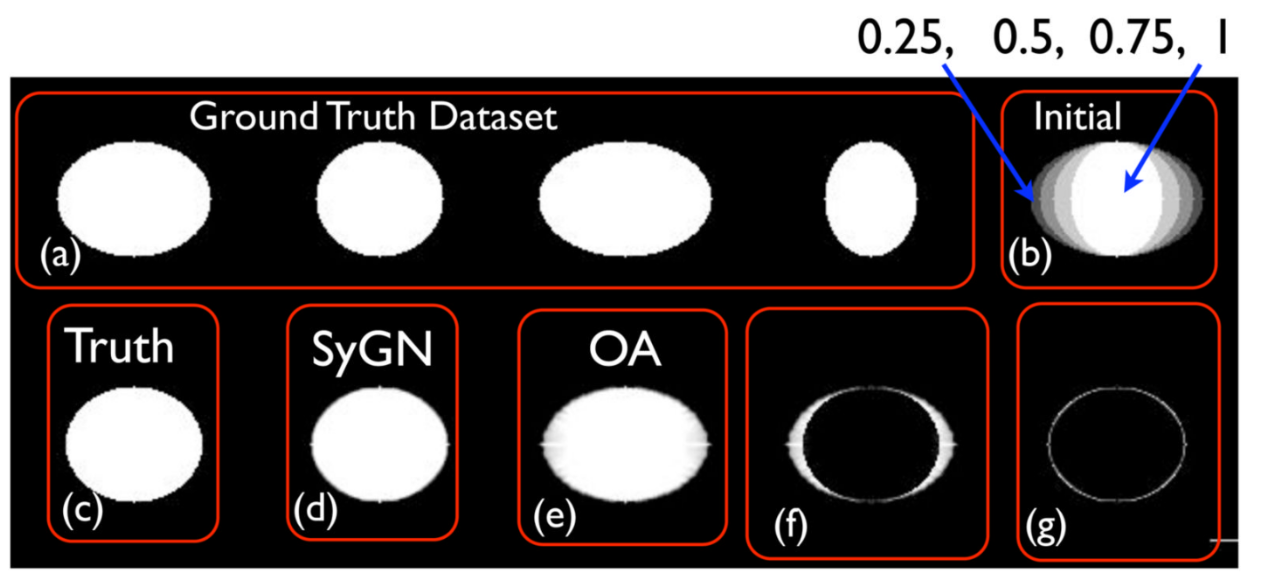
\includegraphics[width=0.8\textwidth]{figures/sygn_ellipses.png}  % Fig. 3 of avants2010sygn
  \caption{Effect of the shape update on binary images. (a)~Four binary
  ellipses; (b)~their initial average, with grey levels $0.25$--$1$;
  (c)~true mean shape; (d)~SyGN result with shape update; (e)~result without
  shape update (appearance only), which converges to the wrong shape;
  (f,g)~errors of (e) and (d) with respect to (c). Reproduced from
  \citet{avants2010sygn}, Fig.~3.}
  \label{fig:sygn_ellipses}                            % referenced in the paragraph above
\end{figure}

\paragraph{Iterations and convergence.}  % how many loops and how to check them
The loop was run for a fixed number of $8$ iterations (the ANTsPy default is
$3$). \citet{avants2010sygn} report that SyGN typically converges in fewer than
ten iterations, usually three to five, depending on the complexity of the
deformations. No stopping criterion is applied by the code. However, ANTsPy
prints the mean absolute value of the average displacement field $W^{(k)}$ at
every iteration; by Eq.~\eqref{eq:frechet_condition} this quantity should tend
towards zero as the template approaches the population mean, and it can be used
to assess convergence.
% TODO: report the 8 printed values of mean |W| from the log (table or plot),
% TODO: e.g. "decreased from ... mm to ... mm", to support the choice of 8 iterations.

\paragraph{Unbiasedness and its limits.}  % what the claims mean for this run
In principle SyGN gives a template that is unbiased: it requires no
user-selected reference, uses a symmetric pairwise method, and centres the
template shape on the population. In the present implementation this holds for
the template shape up to three qualifications: the template grid is inherited
from the first input volume (Eq.~\eqref{eq:initial_template}); the eight volumes
are a small random subset of the two datasets; and the registrations and the
appearance use MI and a sharpened mean instead of the cross-correlation model of
the reference publications.

\paragraph{Output.}  % what the code writes
After the eighth iteration, the template $T^{(8)}$ was written to
\texttt{template.nii.gz}. It is the reference used in
\secref{sec:affine}. The complete procedure is summarised in
Figure~\ref{fig:template_pipeline}.

\begin{figure}[htbp]             % float: LaTeX picks the best spot
  \centering                     % centre the diagram
  \begin{tikzpicture}[
      node distance=4mm,                                 % vertical gap between steps
      box/.style={draw, rounded corners=2pt, align=center,
                   text width=7.5cm, inner sep=4pt, font=\small},  % one box per step
      arr/.style={-{Stealth[length=2mm]}}]               % arrow style
    \node[box]                        (in)   {Random selection: 4 ATM'22 + 4 AIIB23 segmentations};
    \node[box, below=of in]           (init) {Unaligned mean on the grid of the first volume (Eq.~\ref{eq:initial_template})};
    \node[box, below=8mm of init]     (reg)  {Register each airway to the template\\(centre of mass + affine + \texttt{SyN}, MI)};
    \node[box, below=of reg]          (avg)  {Average the warped airway volumes (Eq.~\ref{eq:average_registered})};
    \node[box, below=of avg]          (shp)  {Shape update: $-\alpha\,$mean warp and inverse mean affine (Eq.~\ref{eq:shape_update})};
    \node[box, below=of shp]          (bld)  {Blend with sharpened template, $\beta=0.75$ (Eq.~\ref{eq:blending})};
    \node[draw, dashed, rounded corners=4pt, inner sep=6pt,
          fit=(reg)(bld), label={[font=\small\itshape]right:$\times 8$}] (loop) {};  % the iteration block
    \node[box, below=8mm of bld]      (tpl)  {Final template (\texttt{template.nii.gz})};
    \foreach \a/\b in {in/init, init/reg, reg/avg, avg/shp, shp/bld, bld/tpl}
      \draw[arr] (\a) -- (\b);                           % straight arrows down the chain
    \draw[arr] (bld.west) -- ++(-6mm,0) |- (reg.west);   % loop back: next iteration
  \end{tikzpicture}
  \caption{Groupwise template construction with \texttt{ants.build\_template}.
  The dashed block is one SyGN iteration, repeated eight times.}
  \label{fig:template_pipeline}  % referenced in the Output paragraph
\end{figure}

The NIfTI geometry defines where each original voxel grid lies in physical
space, whereas the affine and diffeomorphic transformations estimated by ANTs
establish anatomical correspondence between these physical domains. The final
template is therefore a population-derived coordinate space in which the
anatomical variability of the eight airway trees has been brought into
correspondence.
